% document setup
\documentclass[12pt,a4paper]{article}
\usepackage[utf8]{inputenc}
\usepackage[ngerman]{babel}

% maths
\usepackage{amsfonts}
\usepackage{amssymb}
\usepackage{amsmath}

% utility
\usepackage{xcolor}
\usepackage{float}
\usepackage[colorlinks=false,linkbordercolor=red,urlbordercolor=red]{hyperref}
\usepackage{caption}
\usepackage[shortlabels]{enumitem}
\usepackage{tikz}

% useful commands
\newcommand{\qed}{\null\nobreak\hfill\square}

% title, author etc.
\title{Analysis I, Blatt 3}
\author{
    Gruppe 11\\
    Lorenz Bung (Matr.-Nr. 5113060)\\
    \href{mailto:lorenz.bung@students.uni-freiburg.de}{\texttt{lorenz.bung@students.uni-freiburg.de}}\\
    Charlotte Rothhaar (Matr.-Nr. 4315016)\\
    \href{mailto:charlotte.rothhaar97@gmail.com}{\texttt{charlotte.rothhaar97@gmail.com}}
}
\date{\today}

% begin document
\begin{document}

\maketitle


\section*{Aufgabe 9}

\begin{enumerate}[(i)]
    \item \begin{enumerate}[(a)]
        \item $(a_n = n - \frac{1}{n})_{n > 0}$\\

        \textbf{Monotonie}.\\
        Behauptung: $(a_n)_{n>0}$ ist monoton steigend.\\
        zu zeigen: $a_{n+1} \geq a_n\ \forall n>0$.\\
        Beweis: \begin{align*}
            n + 1 - \frac{1}{n+1} &> n - \frac{1}{n}\\
            1 - \frac{1}{n+1} &> - \frac{1}{n}\\
            1 &> -\frac{1}{n} + \frac{1}{n+1}
        \end{align*}
        Da $n \in \mathbb{N}$ ist, ist $|\frac{1}{n}| > |\frac{1}{n+1}|$ und damit $\frac{1}{n+1} - \frac{1}{n} < 0 < 1$.
        Somit ist $(a_n)_{n>0}$ monoton steigend.
        Da nicht nur ``$\geq$'', sondern sogar ``$>$'' gilt, ist $(a_n)_{n>0}$ damit nicht monoton fallend.\\

        \textbf{Konvergenz}.\\
        Behauptung: $\lim\limits_{n \to \infty} (a_n)_{n>0} = \infty$.\\
        Beweis: Wir teilen $a_n$ zunächst in zwei Folgen $(b_n = n)_{n>0}$ und $(c_n = - \frac{1}{n})_{n>0}$ auf.\\

        Behauptung: Die Folge $b_n' := (\frac{1}{b_n})_{n>0}$ konvergiert gegen $0$.\\
        zu zeigen: $\forall \varepsilon > 0\ \exists n_0 \in \mathbb{N}: |b_n' - 0| < \varepsilon\ \forall n \geq n_0$.\\
        Beweis:
        Sei $\varepsilon > 0$.
        Wähle nun $n_0 := \lceil\frac{2}{\varepsilon}\rceil$.\\
        Dann ist $$|b_n' - 0| = |b_n'| = |\frac{1}{n}| = \frac{1}{n} \leq \frac{1}{n_0} = \frac{1}{\frac{2}{\varepsilon}} = \frac{\varepsilon}{2} < \varepsilon.$$\\
        Laut \textit{Lemma 3.3.3.} ist $\lim\limits_{n \to \infty}(b_n)_{n>0} = \infty$, wenn $\lim\limits_{n \to \infty}(\frac{1}{b_n})_{n>0} = \lim\limits_{n \to \infty}(b_n')_{n>0} = 0$.
        Damit ist $\lim\limits_{n \to \infty}(b_n)_{n>0} = \infty$.\\

        Behauptung: Die Folge $(c_n)_{n>0}$ konvergiert mit Grenzwert $0$.\\
        zu zeigen: $\forall \varepsilon > 0\ \exists n_0 \in \mathbb{N}: |c_n - 0| < \varepsilon\ \forall n \geq n_0$.\\
        Beweis:
        Sei $\varepsilon > 0$.
        Wähle nun $n_0 := \lceil\frac{2}{\varepsilon}\rceil$.\\
        Dann ist $$|c_n - 0| = |c_n| = |-\frac{1}{n}| = \frac{1}{n} \leq \frac{1}{n_0} = \frac{1}{\frac{2}{\varepsilon}} = \frac{\varepsilon}{2} < \varepsilon.$$\\
        Damit ist $\lim\limits_{n \to \infty}(c_n)_{n>0} = 0$.\\

        Nach GW-Satz gilt nun $\lim\limits_{n \to \infty}(a_n)_{n>0} = \lim\limits_{n \to \infty}(b_n)_{n>0} + \lim\limits_{n \to \infty}(c_n)_{n>0} = \infty + 0 = \infty$.\\

        \textbf{Beschränktheit}.\\
        Da $\lim\limits_{n \to \infty}(a_n)_{n>0} = \infty$, kann es keine obere Schranke geben.\\
        Da $(a_n)_{n>0}$ monoton wachsend ist, ist $$\inf\ (a_n)_{n>0} = a_1 = 1 - \frac{1}{1} = 0 = \min\ (a_n)_{n>0}.$$


        \item $(b_n = \sqrt{n+1} - \sqrt{n})_n$\\

        \textbf{Monotonie}.\\
        Behauptung: $(b_n)_n$ ist monoton fallend.\\
        zu zeigen: $b_{n+1} \leq b_n\ \forall n > 0$.\\
        Beweis:\begin{align*}
            b_{n+1} &\leq b_n\\
            \sqrt{n+2} - \sqrt{n+1} &\leq \sqrt{n+1} - \sqrt{n}\\
            \sqrt{n+2} &\leq -\sqrt{n} + 2\sqrt{n+1}\\
            \sqrt{n} + \sqrt{n+2} &\leq 2\sqrt{n+1}\\
            n + 2\sqrt{n^2+2n} + n + 2 &\leq 4n + 4\\
            2\sqrt{n^2+2n} &\leq 2n + 2\\
            \sqrt{n^2+2n} &\leq n + 1\\
            n^2 + 2n &\leq n^2 + 2n + 1\\
            0 &< 1.
        \end{align*}
        Da sogar $b_{n+1} < b_n$, ist $(b_n)_n$ streng monoton fallend und kan damit nicht monoton wachsend sein.\\

        \textbf{Konvergenz}.\\
        Behauptung: $\lim\limits_{n \to \infty} (b_n)_n = 0$.\\
        Beweis: Wir teilen $b_n$ in zwei Folgen $(d_n = \sqrt{n+1})_n$ und $(e_n = -\sqrt{n})_n$ auf.\\
        Dann ist $\lim\limits_{n \to \infty}(d_n)_n = \infty$ sowie $\lim\limits_{n \to \infty}(e_n)_n = -\infty$ und damit insgesamt $\lim\limits_{n \to \infty}(b_n)_n = \lim\limits_{n \to \infty}(d_n)_n + \lim\limits_{n \to \infty}(e_n)_n = \infty - \infty = 0$.\\
        Damit konvergiert $(b_n)_n$ gegen den Grenzwert $0$.\\

        \textbf{Beschränktheit}.\\
        Aus Monotonie und Konvergenzverhalten folgen
        $$\sup\ (b_n)_n = b_0 = \sqrt{1} - \sqrt{0} = 1 = \max\ (b_n)_n$$
        und
        $$\inf\ (b_n)_n = \lim\limits_{n \to \infty} (b_n)_n = 0.$$
    \end{enumerate}


    \item \begin{enumerate}[(a)]
        \item \begin{minipage}{\linewidth}
            \centering
            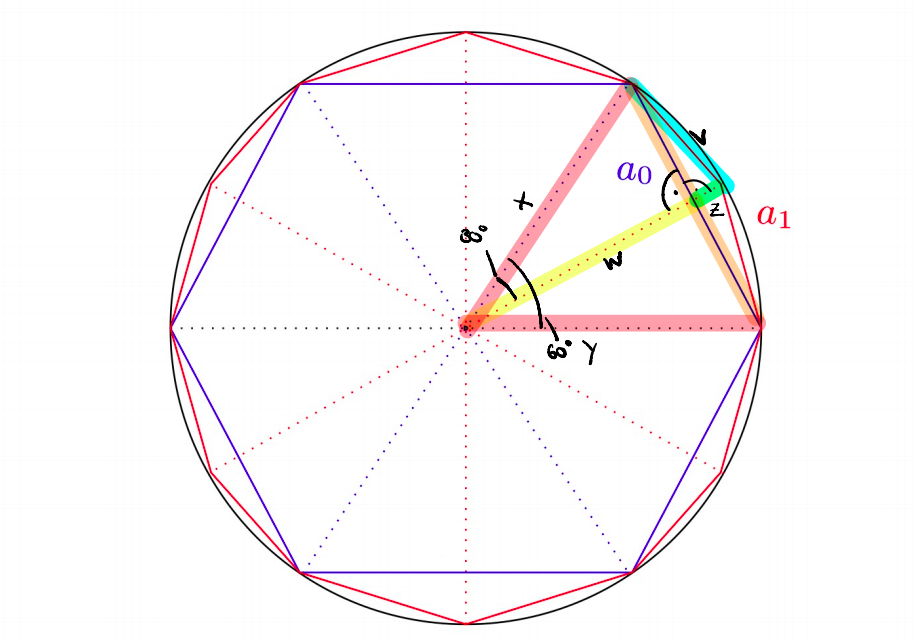
\includegraphics[width=0.75\textwidth]{circle.png}
            \captionof{figure}{}
            \label{fig:a9iia}
        \end{minipage}

        Aus den in \autoref{fig:a9iia} angestellten Überlegungen ergibt sich:
        \begin{align*}
            {a_{n+1}}^2 &= \left(\frac{a_n}{2}\right)^2 + z^2\\
            &= \frac{{a_n}^2}{4} + (1 - w)^2\\
            &= \frac{{a_n}^2}{4} + \left(1 - \sqrt{1 - \frac{a^2}{4}}\right)^2\\
            &= \frac{{a_n}^2}{4} + \left(1 - 2\sqrt{1 - \frac{{a_n}^2}{4}} + 1 - \frac{{a_n}^2}{4}\right)\\
            &= \frac{{a_n}^2}{4} + 2 - 2\sqrt{\frac{4 - {a_n}^2}{4}} - \frac{{a_n}^2}{4}\\
            {a_{n+1}}^2 &= 2 - \sqrt{4 - {a_n}^2}\\
            a_{n+1} &= \sqrt{2 - \sqrt{4 - {a_n}^2}}.
        \end{align*}
        $\qed$

        \item \begin{minipage}{\linewidth}
            \centering
            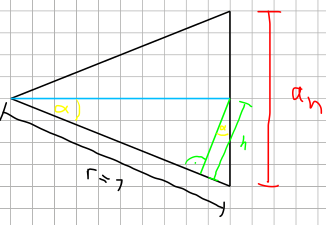
\includegraphics[width=0.66\textwidth]{triangle.png}
            \captionof{figure}{}
            \label{fig:a9iib}
        \end{minipage}

        Aus den in \autoref{fig:a9iib} angestellten Überlegungen ergibt sich
        $h = \cos \left(\frac{30^{\circ}}{2^n}\right) \frac{a_n}{2}$
        und
        $A_{\Delta} = \frac{1}{2}rh = \frac{1}{2}\cos\left(\frac{30^{\circ}}{2^n}\right) \frac{a_n}{2}$.
        Da das das Sechseck ($V_0$) $12$ solcher Dreiecke enthält, ergibt sich für die Gesamtfläche
        \begin{align*}
            f_n &= 12 * 2^n * \frac{1}{2} * \cos\left(\frac{30^{\circ}}{2^n}\right) \frac{a_n}{2}\\
            &= 3 * 2^n * \cos\left(\frac{30^{\circ}}{2^n}\right) a_n\\
            &= 6 * 2^n * \cos\left(\frac{30^{\circ}}{2^n}\right) * \sin\left(\frac{30^{\circ}}{2^n}\right)\\
            f_n &= 3 * 2^n * \sin\left(\frac{60^{\circ}}{2^n}\right).
        \end{align*}


        \item $f_n$ ist konvergent, falls $f_n$ monoton wachsend und von oben beschränkt ist.\\

        \textbf{Monotonie}.\\
        Behauptung: $f_n$ ist monoton wachsend.\\
        zu zeigen: $f_{n+1} \geq f_n$\\
        Beweis: Angenommen, $f_{n+1} \geq f_n$ gilt.
        Dann ist
        \begin{align*}
            f_{n+1} &\geq f_n\\
            3 * 2^{n+1} * \sin\left(\frac{60^{\circ}}{2^{n+1}}\right) &\geq 3 * 2^n * \sin\left(\frac{60^{\circ}}{2^n}\right)\\
            2\sin\left(\frac{60^{\circ}}{2^n*2}\right) &\geq \sin\left(\frac{60^{\circ}}{2^n}\right)\\
            2\sin\left(\frac{30^{\circ}}{2^n}\right) &\geq \sin\left(\frac{60^{\circ}}{2^n}\right)\\
            2\sin(30^{\circ}) &\geq \sin(60^{\circ})\\
            1 &\geq 0,866...
        \end{align*}
        Somit ist $f_n$ monoton wachsend.\\

        \textbf{Beschränktheit}.\\
        Behauptung: $\pi$ ist obere Schranke von $f_n$.\\
        zu zeigen: $\pi \geq f_n\ \forall n \in \mathbb{N}$.\\
        Beweis: Angenommen, die Behauptung ist wahr.
        Dann ist
        \begin{align*}
            \pi &\geq f_{n+1}\\
            \pi &\geq 3 * 2^{n+1} * \sin\left(\frac{60^{\circ}}{2^{n+1}}\right)\\
            \frac{\pi}{2^n} &\geq 3 * 2 * \sin\left(\frac{30^{\circ}}{2^n}\right).
        \end{align*}
        Für $n \to \infty$ verhalten sich beide Seiten gleich, daher kann $n$ einen beliebigen Wert annehmen.
        Somit ist
        \begin{align*}
            \pi &\geq 6 * \sin(30^{\circ})\\
            \pi &\geq 3.
        \end{align*}
        Damit ist $f_n$ durch $\pi$ von oben beschränkt.\\
        Insgesamt ist $f_n$ monoton wachsend und von oben beschränkt und damit konvergent.\\
        $\qed$
    \end{enumerate}
\end{enumerate}


\section*{Aufgabe 10}

\begin{enumerate}[(i)]
    \item Da die Folge $(a_n)_n$ aus den endlos wiederholten Folgengliedern $0, 1, 2, 1$ besteht, sind die Häufungspunkte $0$ und $2$.\\
    Damit ist $\liminf\limits_{n \to \infty} a_n = 0$ und $\limsup\limits_{n \to \infty} a_n = 2$.\\

    $(b_n)_n$ besteht aus der Wiederholung von $2, 1, 1, 0$.
    Damit sind auch hier $0$ und $2$ Häufungspunkte.\\
    Weiterhin sind $\liminf\limits_{n \to \infty} b_n = 0$ und $\limsup\limits_{n \to \infty} b_n = 2$.\\

    Die Folge $(c_n)_n := (a_n + b_n)_n$ besteht somit aus einer endlosen Wiederholung der Folgenglieder $a_0 + b_0, \dots, a_4 + b_4$, also $2, 2, 3, 1$.
    Die Häufungspunkte sind also $1$ und $3$, $\liminf\limits_{n \to \infty} c_n = 1$ und $\limsup\limits_{n \to \infty} c_n = 3$.

    \item Sei $a_n$ reelle eine Folge.\\
    zu zeigen: $\limsup\limits_{n \to \infty} (-a_n) = -\liminf\limits_{n \to \infty} a_n$.\\
    Beweis:\\
    Da $\limsup\limits_{n \to \infty} (-a_n) =: x$ existiert, muss es eine Teilfolge $(a_{n_m})_m$ geben, die gegen $x$ konvergiert.
    Wegen $\lim\limits_{m \to \infty} (-a_{n_m}) = - \lim\limits_{m \to \infty} a_{n_m}$ ist auch $-x$ ein Häufungspunkt.\\
    Dieser muss minimal sein:
    Für alle Häufungspunkte $y$ von $(a_{n_m})_m$ muss gelten, dass $\lim\limits_{m \to \infty} a_{n_m} = \lim\limits_{m \to \infty} -(-a_{n_m}) = - \lim\limits_{m \to \infty} -a_{n_m} = -y$.
    Wegen $-x = \limsup\limits_{n \to \infty} a_n$ ist $-y \leq -x \Leftrightarrow y \geq x$.\\
    Damit ist $x$ der kleinste Häufungspunkt von $(a_{n_m})_m$ und $\limsup\limits_{n \to \infty} (-a_n) = - \liminf\limits_{n \to \infty} a_n$.\\
    $\qed$

    \item
\end{enumerate}


\section*{Aufgabe 11}

\begin{enumerate}[(i)]
    \item Beweis durch Widerspruch:\\
    Angenommen, $f$ hätte mehr als einen Fixpunkt.
    Seien diese Fixpunkte $x,y \in I$.\\
    Dann ist
    $|f(x) - f(y)| < q|x - y|$ und nach Definition somit\\
    $|x - y| < q|x - y|$ bzw. $1 < q$.
    Widerspruch, da $q \in (0, 1)$!\\
    $\qed$

    \item Gegeben sei die Folge $(x_n)_n$ mit $x_{n+1} = f(x)$.\\
    Ist diese Folge eine Cauchyfolge, so konvergiert sie auch gegen einen Grenzwert $x'$ mit $f(x') = x'$.\\
    Es gilt:
    \begin{equation}
        \label{eq:a11i1}
        q * |x_n - x_{n-1}| = q * |f(x_{n-1}) - f(x_{n-2})| \leq q * q * |x_{n-1} - x_{n-2}|
    \end{equation}
    und damit
    \begin{align*}
        |x_{n+1} - x_n| &= |f(x_n) - f(x_{n-1})|\\
        &\leq q * |x_n - x_{n-1}|\\
        &\overset{\text{(\ref{eq:a11i1})}}{\leq} q^2 * |x_{n-1} - x_{n-2}|\\
        &\ \ \vdots\\
        &\leq q^n * |x_1 - x_0|.
    \end{align*}
    Somit ist
    $$|x_{n+m+n} - x_{n+m}| \leq q^m * |x_{n+1} - x_n|.$$
    Mithilfe der Dreiecksungleichung erhalten wir
    \begin{align*}
        |x_{n+m} - x_n| \overset{\Delta\text{-Ugl.}}{\leq} &|x_{n+m} - x_{n+m+n}| + |x_{n+m-1} - x_{n+m-2}|\\
        &\qquad\vdots\\
        &|x_{n+1} - x_n|.
    \end{align*}
    Es folgt:
    \begin{align*}
        |x_{n+m} - x_n| &\leq q^{m-1}|x_{n+1}-x_n|+q^{m-2}|x_{n+1}-x_n|+\dots+q^0|x_{n+1}-x_n|\\
        &= \left(\sum\limits_{i=0}^{m-1}q^i\right)|x_{n+1}-x_n|\\
        &\leq \left(\sum\limits_{i=0}^{\infty}q^i\right)|x_{n+1}-x_n|\\
        &= \frac{1}{1-k}*q^n|x_1-x_0| \overset{n \to 0}{\longrightarrow} 0.
    \end{align*}
    Damit ist $(x_n)_n$ eine Cauchyfolge und konvergiert.\\
    Weiterhin gilt für den Grenzwert $x$ der Folge
    $$x = \lim\limits_{n \to \infty}x_n = \lim\limits_{n \to \infty}x_{n+1} = \lim\limits_{n \to \infty}f(x_n) = f(x_n).$$
    Damit ist der Grenzwert $x$ der Fixpunkt $x'$.\\
    $\qed$

    \item
\end{enumerate}


\section*{Aufgabe 12}

\begin{enumerate}[(i)]
    \item Sei $a \in \mathbb{R},\ a > 0$.
    Dann ist
    $$a + \frac{1}{a} = \frac{a^2}{a} + \frac{1}{a} = \frac{a^2 + 1}{a} \geq 2$$
    und somit
    $$\frac{a^2 + 1}{a} -2 = \frac{a^2+1}{a} - \frac{2a}{a} = \frac{a^2 -2a +1}{a} = \frac{(a-1)^2}{a} \geq 0.$$
    $(a-1)^2$ muss schon positiv sein (denn $x^2 \geq 0 \forall x \in \mathbb{R}$), und wegen $a > 0$ folgt auch $\frac{(a-1)^2}{a} \geq 0$.\\
    $\qed$

    \item
    \item Es ist
    \begin{equation}
        \label{eq:a12iii1}
        x_n \geq x_{n+1}
    \end{equation}
    und somit
    \begin{equation}
        \label{eq:a12iii2}
        \frac{c}{x_n} \leq \frac{c}{x_{n+1}}.
    \end{equation}
    Wegen \autoref{eq:a12iii2} ist damit $\left[\frac{c}{x_{n+1}}, x_n\right] \subseteq \left[\frac{c}{x_n}, x_n\right]$.
    Weil außerdem wegen \autoref{eq:a12iii1} $\left[\frac{c}{x_n}, x_{n+1}\right] \subseteq \left[\frac{c}{x_n}, x_n\right]$ ist, muss der Schnitt $\left[\frac{c}{x_{n+1}}, x_{n+1}\right]$ dieser beiden Intervalle auch eine Teilmenge von $\left[\frac{c}{x_n}, x_n\right]$ sein.\\
    $\qed$

    \item
    \item
\end{enumerate}

% end document
\end{document}